\chapter{Quantifying and Visualizing the Quality of a Mixed-Bag Solver Output}\label{sec:quantifyingSolverQuantify}

Modern jig swap puzzle solvers are not able to perfectly reconstruct the ground-truth input in most cases.  As such, quantifiable metrics are required to objectively compare the quality of outputs from different solvers.  Cho~\textit{et al.}~\cite{cho2010} defined two such metrics namely: direct accuracy and neighbor accuracy. These metrics have been used by others including \cite{sholomon2013, pomeranz2011, paikin2015, son2014, gallagher2012}.  This section describes the existing quality metrics, their weaknesses, and proposes enhancements to these metrics to make them more meaningful for Type~2 and Mixed-Bag puzzles.  This thesis also proposes advanced metrics for quantifying the best buddy attributes of an image.

In the final section, tools developed as part of this thesis to visualize the solver output quality are discussed.

\section{Direct Accuracy}\label{sec:directAccuracy}

Direct accuracy is a relatively na\"{\i}ve quality metric; it is defined as the fraction of pieces placed in the same location in both the ground-truth (i.e., original) and solved image with respect to the total number of pieces.  Equation~\eref{eq:directAccuracy} shows the formal definition of direct accuracy ($DA$), where $n$ is the total number of pieces and $c$ is the number of pieces in the solved image that are placed in their original (i.e., correct) location.

\begin{equation} \label{eq:directAccuracy}
DA = \frac{c}{n}
\end{equation}

Direct accuracy is vulnerable to shifts in the solved image where even a few misplaced pieces can cause a significant decrease in accuracy.  As shown in Figure~\ref{fig:directAccuracyOnePieceEffect}, this can be particularly true when the ground-truth image's dimensions are not known by the solver.

This thesis proposes two new direct accuracy metrics namely: Enhanced Direct Accuracy Score (EDAS) and Shiftable Enhanced Direct Accuracy Score (SEDAS).  They are described in the following two subsections; the complementary relationship between EDAS and SEDAS is described in the third subsection.

\subsection{Enhanced Direct Accuracy Score}\label{sec:enhancedDirectAccuracyScore}

The standard direct accuracy metric does not account for the possibility that there may be pieces from multiple input puzzles in the same solver output image.  For a given a puzzle $P_i$ in the set of input puzzles $P$ (i.e., $P_i \in P$) and a set of solved puzzles $S$ where $S_j$ is in $S$, Enhanced Direct Accuracy Score (EDAS) is defined as shown in Equation~\eref{eq:enhancedDirectAccuracyScore}.  $c_{ij}$ is the number of pieces from input puzzle $P_i$ correctly placed (with no rotation for Type~2 puzzles) in solved puzzle $S_j$ while $n_i$ is the number of pieces in puzzle $P_i$. $m_{k,j}$ is the number of pieces from an input puzzle $P_k$ (where $k \ne i$) that are also in $S_j$.

\begin{equation} \label{eq:enhancedDirectAccuracyScore}
EDAS_{P_i} = \argmax_{S_j \in S}\frac{c_{i,j}}{n_i + \sum_{k \ne i}(m_{k,j})}
\end{equation}


Standard direct accuracy (see Equation~\eref{eq:directAccuracy}) and EDAS are equivalent when solving a single puzzle. For Mixed-Bag solvers, EDAS necessarily marks as incorrect any pieces from $P_i$ that are not in $S_j$ by dividing by $n_i$.  What is more, the summation of $m_{k,j}$ in EDAS penalizes for any puzzle pieces in the solver output $S_j$ that are not from input puzzle $P_i$.  Therefore, EDAS takes into account both extra and missing pieces in the solver output.

It is important to note that EDAS is a score and not a measure of accuracy. While its value is bounded between 0 and 1 (inclusive), it is not specifically defined as the number of correct placements divided by the total number of placements since the denominator of Equation~\eref{eq:enhancedDirectAccuracyScore} is greater than or equal to the number of pieces in both $P_i$ and $S_j$.

\subsection{Shiftable Enhanced Direct Accuracy Score}\label{sec:shiftableEnhancedDirectAccuracy}

As mentioned previously, the direct accuracy decreases if there are shifts in the solved image.  In many cases such, direct accuracy is overly punitive. 

Figure~\ref{fig:directAccuracyOnePieceEffect} shows a ground-truth image and an actual solver output when the puzzle boundaries were not fixed.  Note that only a single piece is misplaced; this shifted all other pieces to the right one location causing the direct accuracy to drop to zero.  Had this same piece been misplaced along either the right or bottom side of the image, the direct accuracy would have been largely unaffected.  The fact that direct accuracy can give such vastly differing results for essentially the same error shows that direct accuracy has a fundamental flaw.  This thesis proposes Shiftable Enhanced Direct Accuracy Score (SEDAS) to address the often misleadingly punitive nature of standard direct accuracy. 

\begin{figure}
\centering
  \begin{tabular}{ >{\centering\arraybackslash}m{2.2in} >{\centering\arraybackslash}m{2.2in} }
	\fbox{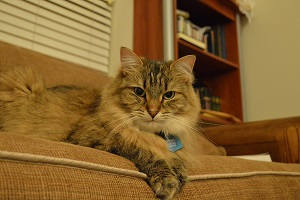
\includegraphics[width=48mm]{./images/muffins_300x200.jpg}} & \fbox{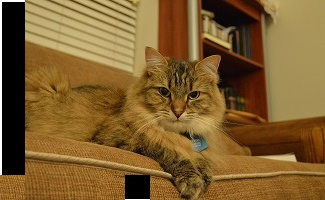
\includegraphics[width=50.1mm]{./images/muffins_300x200_type1}}
	\\ ~\\
	(a) Ground-Truth Image & (b) Solver Output
	\\ ~\\
  \end{tabular}
\caption{Solver Output where a Single Misplaced Piece Catastrophically Affects the Direct Accuracy}
\label{fig:directAccuracyOnePieceEffect}
\end{figure}

Equation~\eref{eq:shiftableEnhancedDirectAccuracyScore} is the formal definition of $SEDAS$.  $d_{min}$ represents the Manhattan distance between the upper left corner of the solved image and the nearest placed puzzle piece.  Similarly, $L$ is the set of all puzzle piece locations within radius $d_{min}$ (inclusive) of the upper left corner of the image.  Given that $l$ is a location in $L$ that is used as the reference point for determining the absolute location of all pieces, then SEDAS is defined as shown in Equation~\eref{eq:shiftableEnhancedDirectAccuracyScore}.  

\begin{equation} \label{eq:shiftableEnhancedDirectAccuracyScore}
SEDAS_{P_i} = \argmax_{l \in L} \bigg( \argmax_{S_j \in S}\frac{c_{i,j,l}}{n_i + \sum_{k \ne i}(m_{k,j})} \bigg)
\end{equation}

\noindent
In the standard definition of direct accuracy proposed by Cho \textit{et al.}, $l$ is fixed at the upper left corner of the image.  In contrast, SEDAS shifts this reference point within a radius of the upper left corner of the image in order to find a more meaningful value for direct accuracy. 

Rather than defining SEDAS based off the distance $d_{min}$, an alternative approach is to use the point anywhere in the image that maximizes Equation~\eref{eq:shiftableEnhancedDirectAccuracyScore}.  However, that approach can take significantly longer to compute in particular when the solved puzzle has several thousand pieces.  SEDAS balances the need for a meaningful direct accuracy score against computation efficiency.

\subsection{The Necessity to Use Both EDAS and SEDAS}\label{sec:importanceEdasSedas}

While EDAS can be misleadingly punitive, it cannot be wholly replaced by SEDAS.  Rather, EDAS and SEDAS serve complementary roles.  First, EDAS must necessarily be calculated as part of SEDAS since the upper left corner location is inherently a member of the set $L$.  Hence, there is no additional time required to calculate EDAS.  What is more, by continuing to use EDAS along with SEDAS, some shifts in the solved image may be quantified; this would not be possible if SEDAS was used alone.

\section{Neighbor Accuracy}\label{sec:neighborAccuracy}

Cho~\textit{et al.}~\cite{cho2010} defined neighbor accuracy as the ratio of the number of puzzle piece sides adjacent to the same piece's side in both the ground-truth and solved image versus the total number of puzzle piece sides.  Formally, let $q$ be the number of sides each piece has (i.e., four in a jig swap puzzle) and $n$ be the number of pieces.  If $a$ is the number of puzzle piece sides adjacent in both the ground-truth and solved images, then the neighbor accuracy, $NA$, is defined as shown in Equation~\eref{eq:neighborAccuracy}.

\begin{equation} \label{eq:neighborAccuracy}
NA = \frac{a}{n~q}
\end{equation}

Unlike direct accuracy, neighbor accuracy is largely unaffected by shifts in the solved image since it considers only a piece's neighbors and not its absolute location.  However, the standard definition of neighbor accuracy cannot encompass the case where pieces from multiple input puzzles may be present in the same solver output.  

\subsection{Enhanced Neighbor Accuracy Score}\label{sec:enhancedNeighborAccuracyScore}

Enhanced Neighbor Accuracy Score (ENAS) improves the neighbor accuracy metric by providing a framework to quantify the quality of Mixed-Bag solver outputs. 

Let $n_i$ be the number of puzzles pieces in the input puzzle $P_i$ and $a_{i,j}$ be the number of puzzle piece sides adjacent in $P_i$ and $S_j$.  If $m_{k,j}$ is the number of puzzle pieces from an input puzzle $P_k$ (where $k \ne i$) in $S_j$, then the ENAS for $P_i$ is defined as shown in Equation~\eref{eq:enhancedNeighborAccuracyScore}.

\begin{equation} \label{eq:enhancedNeighborAccuracyScore}
\ENAS_{P_i} = \argmax_{S_j \in S}\frac{a_{i,j}}{q ~ (n_i + \sum_{k \ne i}(m_{k,j})}
\end{equation}

In the same fashion as the technique described for EDAS in Section~\ref{sec:enhancedDirectAccuracyScore}, ENAS divides by the number of pieces $n_i$ in input puzzle $P_i$.  By doing so, it effectively marks as incorrect any pieces from $P_i$ that are not in $S_j$.  What is more, by including a summation of all $m_{k,j}$ in the denominator of \eref{eq:enhancedNeighborAccuracyScore}, ENAS marks as incorrect any pieces not from $P_i$ that are in $S_j$.  The combination of these two factors allows ENAS to account for extra and misplaced pieces.

\section{Best Buddy Metrics}\label{sec:bestBuddyMetrics}

Chapter~\ref{chap:previousWork} explains that two puzzle pieces are best buddies on their respective sides if they are both more similar to each other than they are to any other pieces.  This thesis refers to a best buddy relationship as ``adjacent'' if the two pieces are neighbors on their respective sides.  In contrast, ``non-adjacent'' best buddies are not neighbors.  It is also possible that a piece has no best buddy at all on one or more sides.

Best buddy relationships have been used for segmentation~\cite{pomeranz2011}, placement~cite{paikin 2015}, and as an estimation metric~\cite{sholomon2013}.  To date, no specific metrics or additional subclassifications of best buddy relationships has been proposed.  The following subsections propose new metrics for studying the best buddy profile of both input and solved puzzles.

\subsection{Interior and Exterior Best Buddies}\label{sec:bestBuddyInteriorExterior}

If an image has fewer non-adjacent best buddies, it means that best buddy relationships become a more accurate determiner of puzzle piece adjacency.  It is expected that a pair of best buddies are more likely to be non-adjacent if they are have no neighbor at all (i.e., the piece(s) is next to an open location like the edge of the image).  This is because those puzzle piece sides have no true neighbor leaving them more inclined to couple with an unrelated piece, which is often another piece's side with no neighbor.  This is illustrated by the example described in Section~\ref{sec:visualizingBestBuddies}.

This thesis subcategorizes non-adjacent best buddies depending on whether they are internal (i.e., the piece has an actual neighbor) or external (i.e., the piece has no neighbor).  Interior non-adjacent best buddies are generally more concerning since they are used for segmentation and potentially as an estimation metric. 

\subsection{Best Buddy Density}\label{sec:bestBuddyDensity}

As mentioned previously, each puzzle piece side may or may not have a best buddy relationship. For a puzzle consisting of $n$ pieces each of which has $q$ sides \footnote{In a jig swap puzzle, $q$ is equal to 4.}, Equation~\eref{eq:bestBuddyDensity} defines the best buddy density, $BBD$ given the image has $b$ total best buddies.   $BBD$ is bounded between 0 and 1 (inclusive); a higher best buddy density indicates that the individual puzzle pieces can be more easily differentiated from one another.  

\begin{equation} \label{eq:bestBuddyDensity}
BBD = \frac{b}{n~q}
\end{equation}

Ideally, a puzzle would have only adjacent best buddies, and that all neighboring puzzle piece sides were also adjacent best buddies.  In such cases, the best buddy density would be less than one; the exact to which it would be below one is dependent on the puzzle dimensions and any missing pieces.  $BBD$ could be further refined to only consider adjacent best buddies in the term $b$.  

Best buddy density may vary across an image with some areas showing lower density than others. Equation~\eref{eq:bestBuddyDensity} can be adjusted to a more local metric by reducing the value of $b$ and $n$ based off the best buddy profile of a connected subset of pieces.

\section{Visualizing Solver Output Quality and Best Buddies Relationships}\label{sec:visualizingSolverAccuracy}

In images with thousands of pieces, it is often difficult to visually determine the location of individual pieces that are incorrectly placed.  What is more, visual tools help developers quickly detect and fix latent bugs.  The following two subsections describe the tools developed as part of this thesis for visualizing direct and neighbor accuracy as well as for visualizing best buddies.

\subsection{Visualizing EDAS and SEDAS}\label{sec:visualizingEdasSedas}

In standard direct accuracy, EDAS, and SEDAS, each puzzle piece is assigned a single value (i.e., correct or incorrect).  Due to that, the direct accuracy visualization represents each puzzle by a square filled with a solid color.  One additional refinement used in this thesis is to subdivide the ``incorrect'' placements into a set of subcategories; they are, in order of precedence: wrong puzzle, wrong location, and wrong rotation.  Table~\ref{tab:directAccuracyColors} shows the colors assigned to puzzle pieces depending on their direct accuracy classification.

\begin{table}[tb]
	\begin{center}
  		\begin{tabular}{ | >{\centering\arraybackslash}m{0.9in} | >{\centering\arraybackslash}m{0.9in} | >{\centering\arraybackslash}m{0.9in} | >{\centering\arraybackslash}m{0.9in} | >{\centering\arraybackslash}m{0.9in} | }
 \hline
    		Wrong Puzzle & Wrong Location & Wrong Rotation & Correct Location  & No Piece Present  \\ \hline
			{\cellcolor{blue}~} & {\cellcolor{red}~}  & {\cellcolor{orange}~}  & {\cellcolor{green}~} & {\cellcolor{black}~}  \\
			{\cellcolor{blue}~} & {\cellcolor{red}~}  & {\cellcolor{orange}~}  & {\cellcolor{green}~} & {\cellcolor{black}~} \\
 \hline
		\end{tabular}
	\end{center}
\caption{Color Scheme for Puzzles Pieces in Direct Accuracy Visualizations}\label{tab:directAccuracyColors}
\end{table}

Figure~\ref{fig:directAccuracyVisualization} shows a Type~2 solver output as well as its associated EDAS and SEDAS visualizations. Since four puzzle pieces were erroneously placed on the left of the image, all but one had the wrong location according to EDAS; the only exception is a single piece that had the right location but wrong rotation.  In contrast, almost all pieces have the correct location in the SEDAS representation; note that the piece in the correct location but wrong rotation in EDAS has the wrong location in SEDAS.

\begin{figure}
\centering
  \begin{tabular}{ >{\centering\arraybackslash}m{2.2in} >{\centering\arraybackslash}m{2.2in} }
  
	\fbox{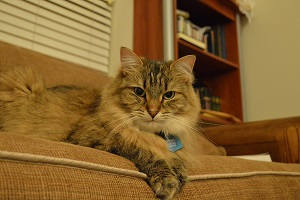
\includegraphics[width=48mm]{./images/muffins_300x200.jpg}} & \fbox{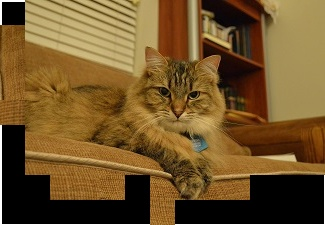
\includegraphics[width=52.1mm]{./images/muffins_300x200_type2}} \\~\\
	(a) Ground-Truth Image & (b) Type~2 Solver Output
\\~\\
	\fbox{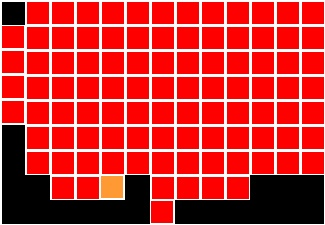
\includegraphics[width=52.1mm]{./images/muffins_300x200_type_EDAS.jpg}} & \fbox{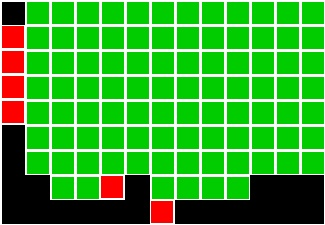
\includegraphics[width=52.1mm]{./images/muffins_300x200_type_SEDAS.jpg}}
\\~\\
	(c) EDAS Visualization & (d) SEDAS Visualization  
  \end{tabular}

\caption{Example Solver Output Visualizations for EDAS and SEDAS}
\label{fig:directAccuracyVisualization}
\end{figure}

\subsection{Visualizing ENAS}\label{sec:visualizingNeighborAccuracy}

In a jig swap puzzle, a piece may have best buddies on up to four sides (since the pieces are square).  As such, each piece in the ENAS visualization is divided into four isosceles triangles; the base of each triangle is along the side of the puzzle piece whose neighbor accuracy is being represented.  A puzzle piece's four isosceles triangles all share a common, non-base vertex at the piece's center.  Table~\ref{tab:neighborAccuracyColors} defines the color assigned to each triangle depending on whether a piece's neighbors in the solver output and ground-truth image match.  The ``wrong puzzle'' classfication applies only to Mixed-Bag puzzles and occurs when a piece in the solver output is does not from the puzzle of interest, $P_i$. 

\begin{table}[t]
\begin{center}
  \begin{tabular}{ | >{\centering\arraybackslash}m{0.9in} | >{\centering\arraybackslash}m{0.9in} | >{\centering\arraybackslash}m{0.9in} | >{\centering\arraybackslash}m{0.9in} | >{\centering\arraybackslash}m{0.9in} | }
 \hline
    Wrong Puzzle & Wrong Neighbor & Correct Neighbor  & No Piece Present  \\ \hline
	{\cellcolor{blue}~} & {\cellcolor{red}~} & {\cellcolor{green}~} & {\cellcolor{black}~}  \\
	{\cellcolor{blue}~} & {\cellcolor{red}~} & {\cellcolor{green}~} & {\cellcolor{black}~}  \\
 \hline
  \end{tabular}
\end{center}
\caption{Color Scheme for Puzzles Piece Sides in Neighbor Accuracy Visualizations}\label{tab:neighborAccuracyColors}
\end{table}

Figure~\ref{fig:neigborAccuracyVisualization} shows an actual output when solving a Mixed-Bag puzzle with two images.  Note that that the puzzle of interest ($P_i$) is the glass and stone building while the other puzzle ($P_k$) is a rainforest house.

\begin{figure}[t]
\centering

  \begin{tabular}{ >{\centering\arraybackslash}m{2.2in} >{\centering\arraybackslash}m{2.2in} }
  
	\fbox{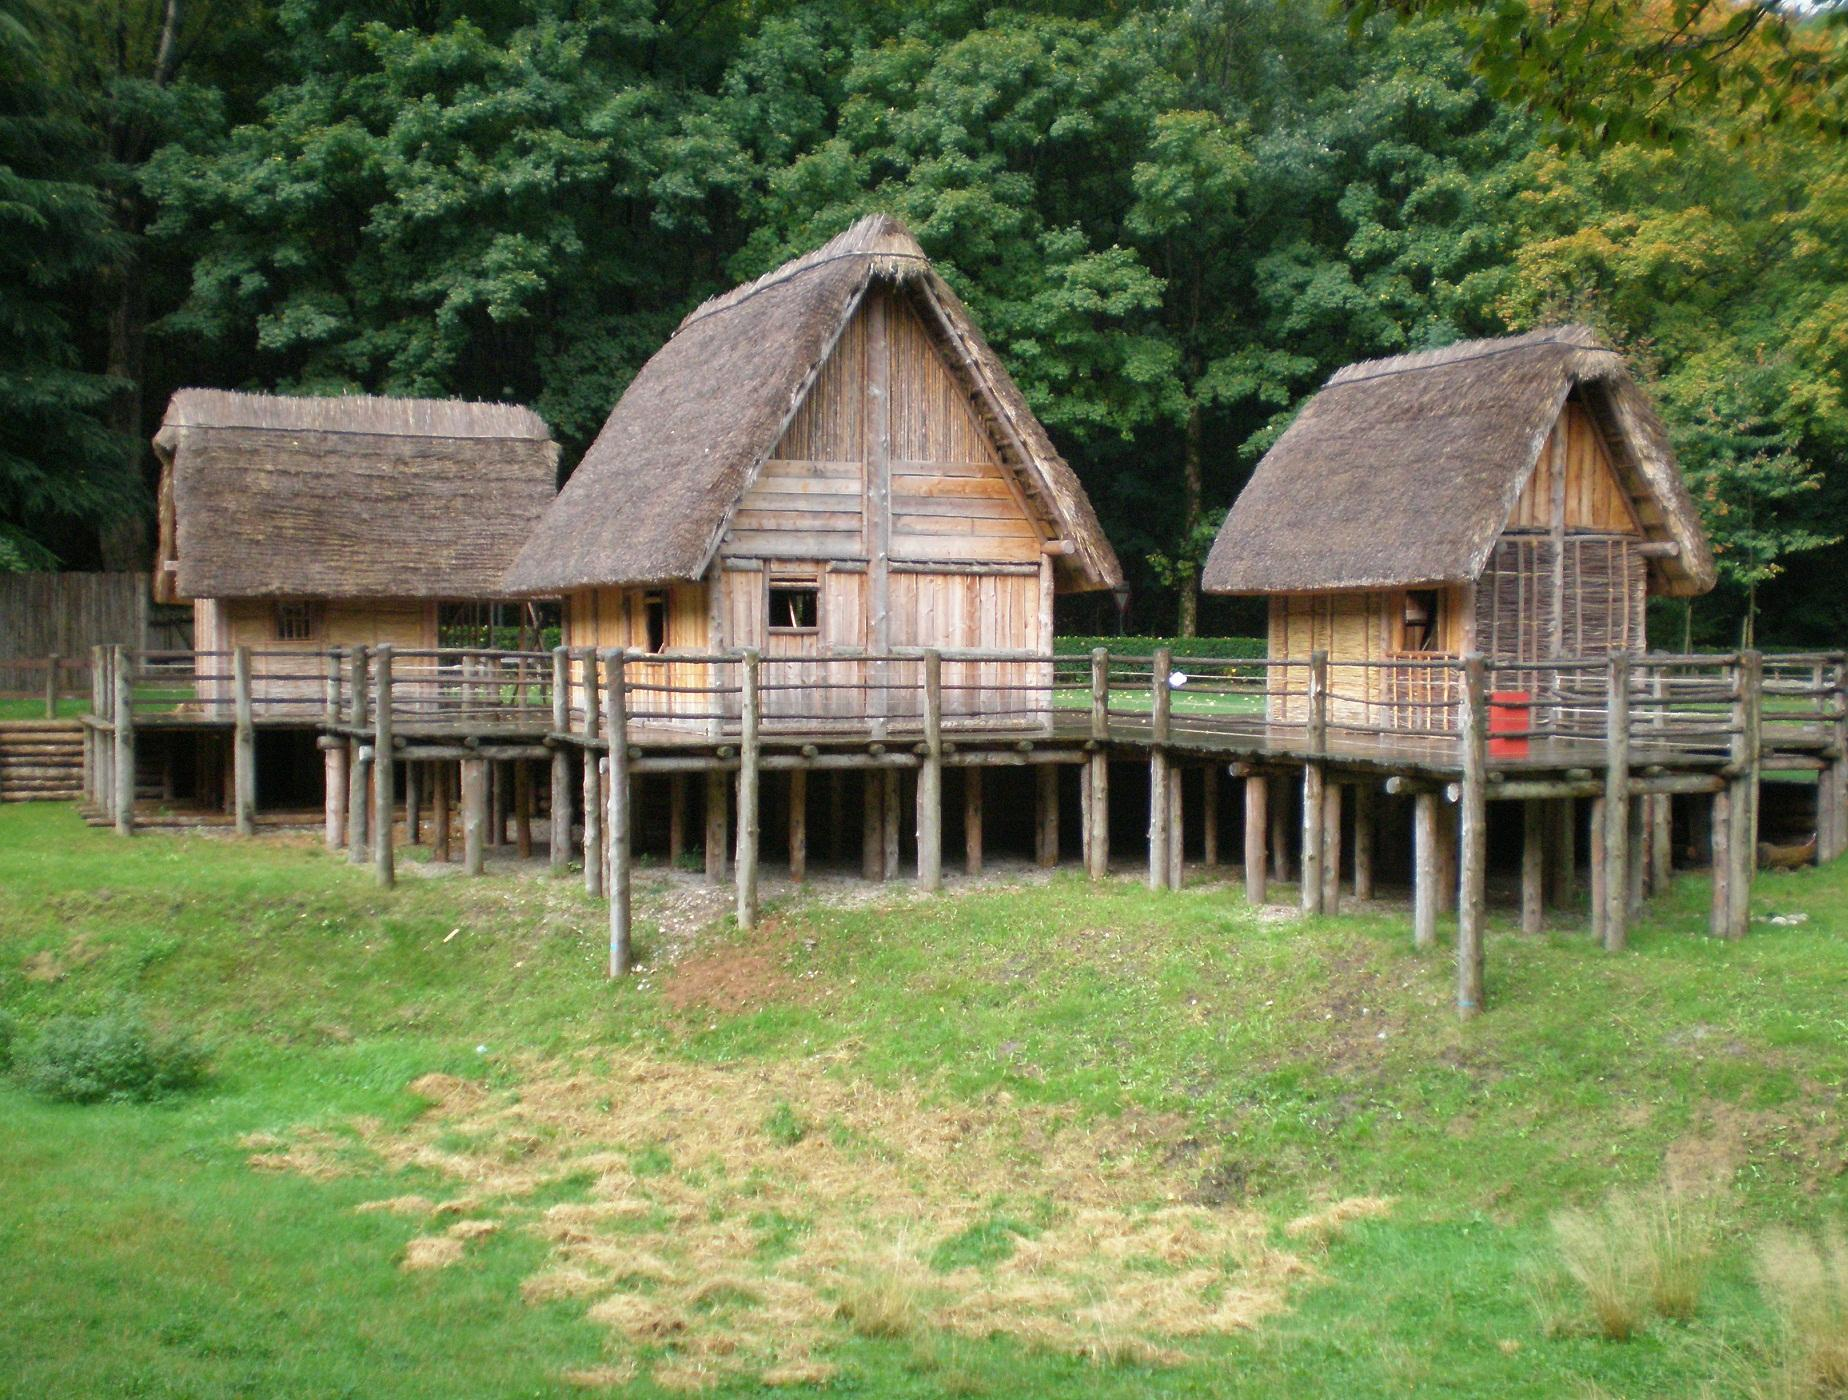
\includegraphics[width=1.7in]{./images/pomeranz_3300_1.jpg}} & \fbox{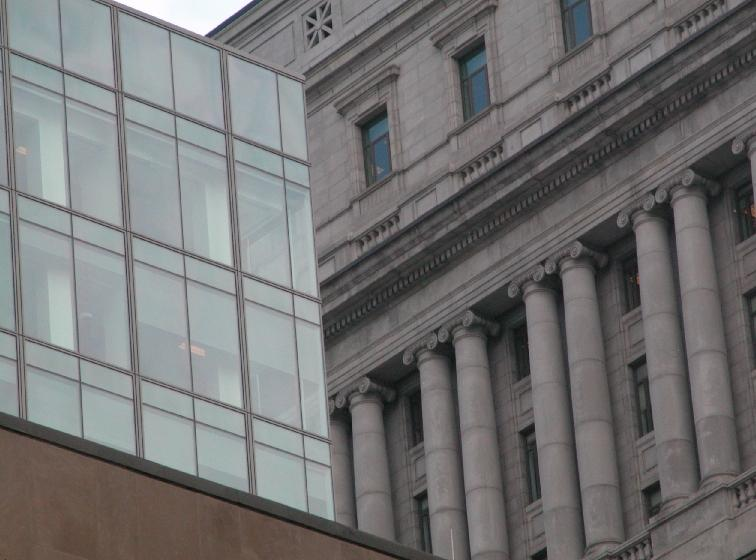
\includegraphics[width=1.5in]{./images/mcgill_20.jpg}} \\~\\
	(a) Input Image \# 1 - Rainforest House \cite{pomeranzBenchmarkImages} & (b) Input Image \# 2 - Building Exterior \cite{mcgillImageDatabase}
\\~\\
	\fbox{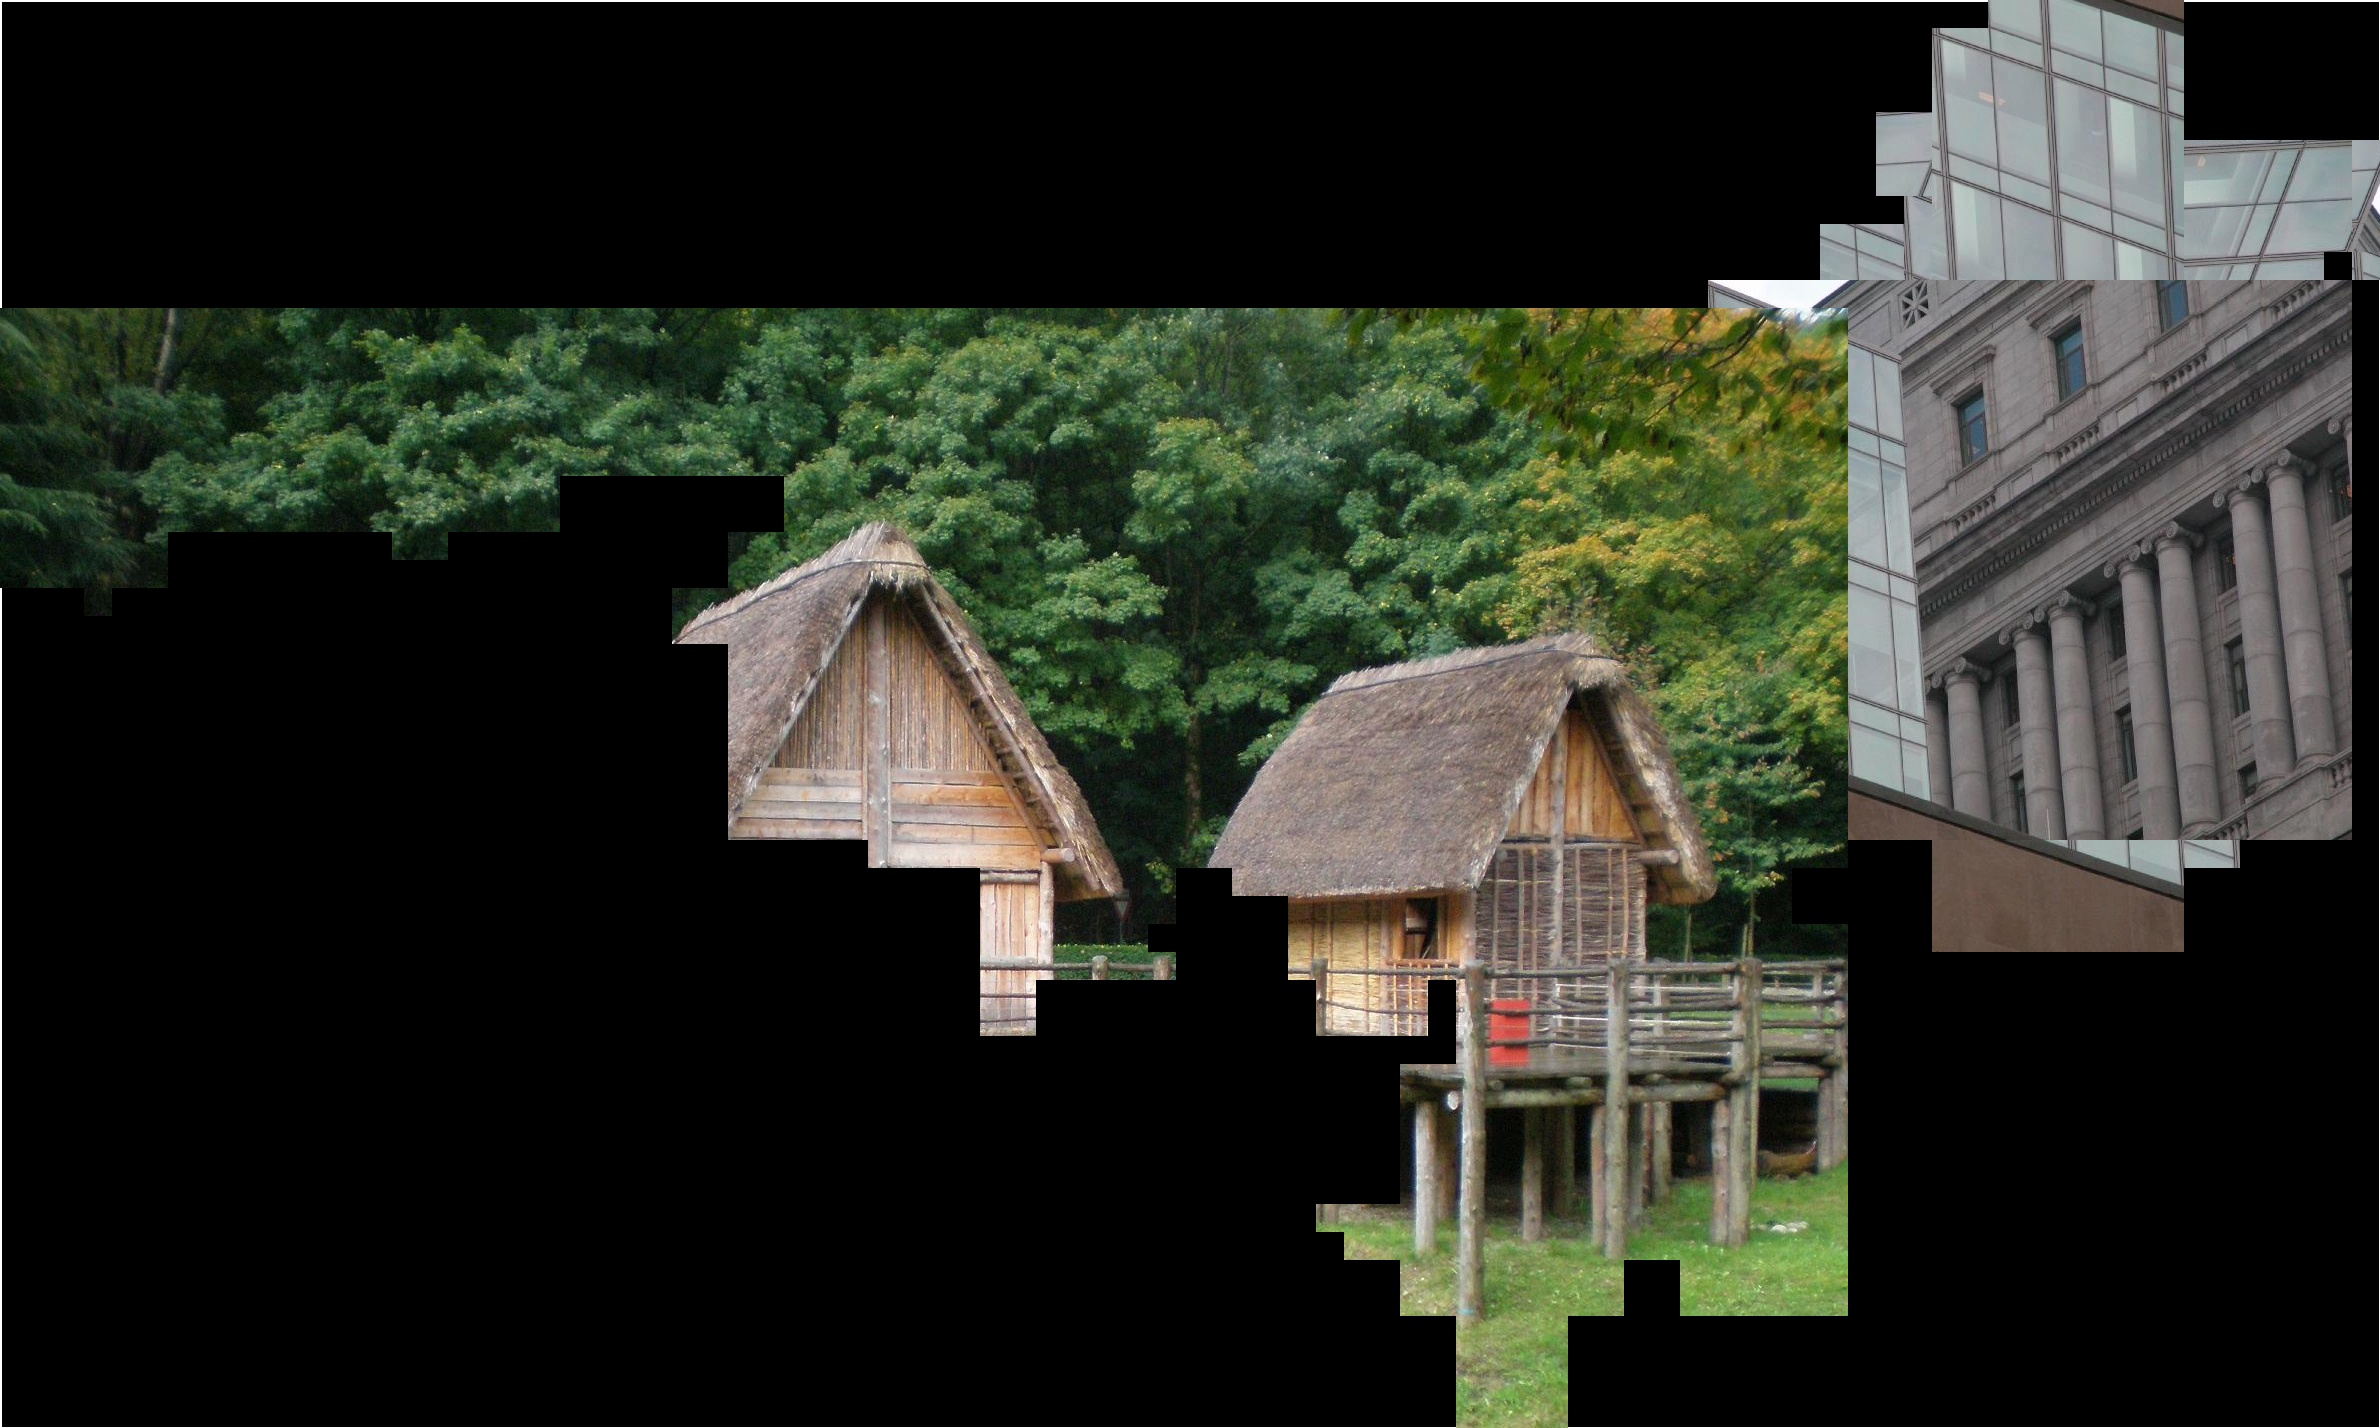
\includegraphics[width=2.1in]{./images/3300_1_mcgill_20_type_2.jpg}}
	& \fbox{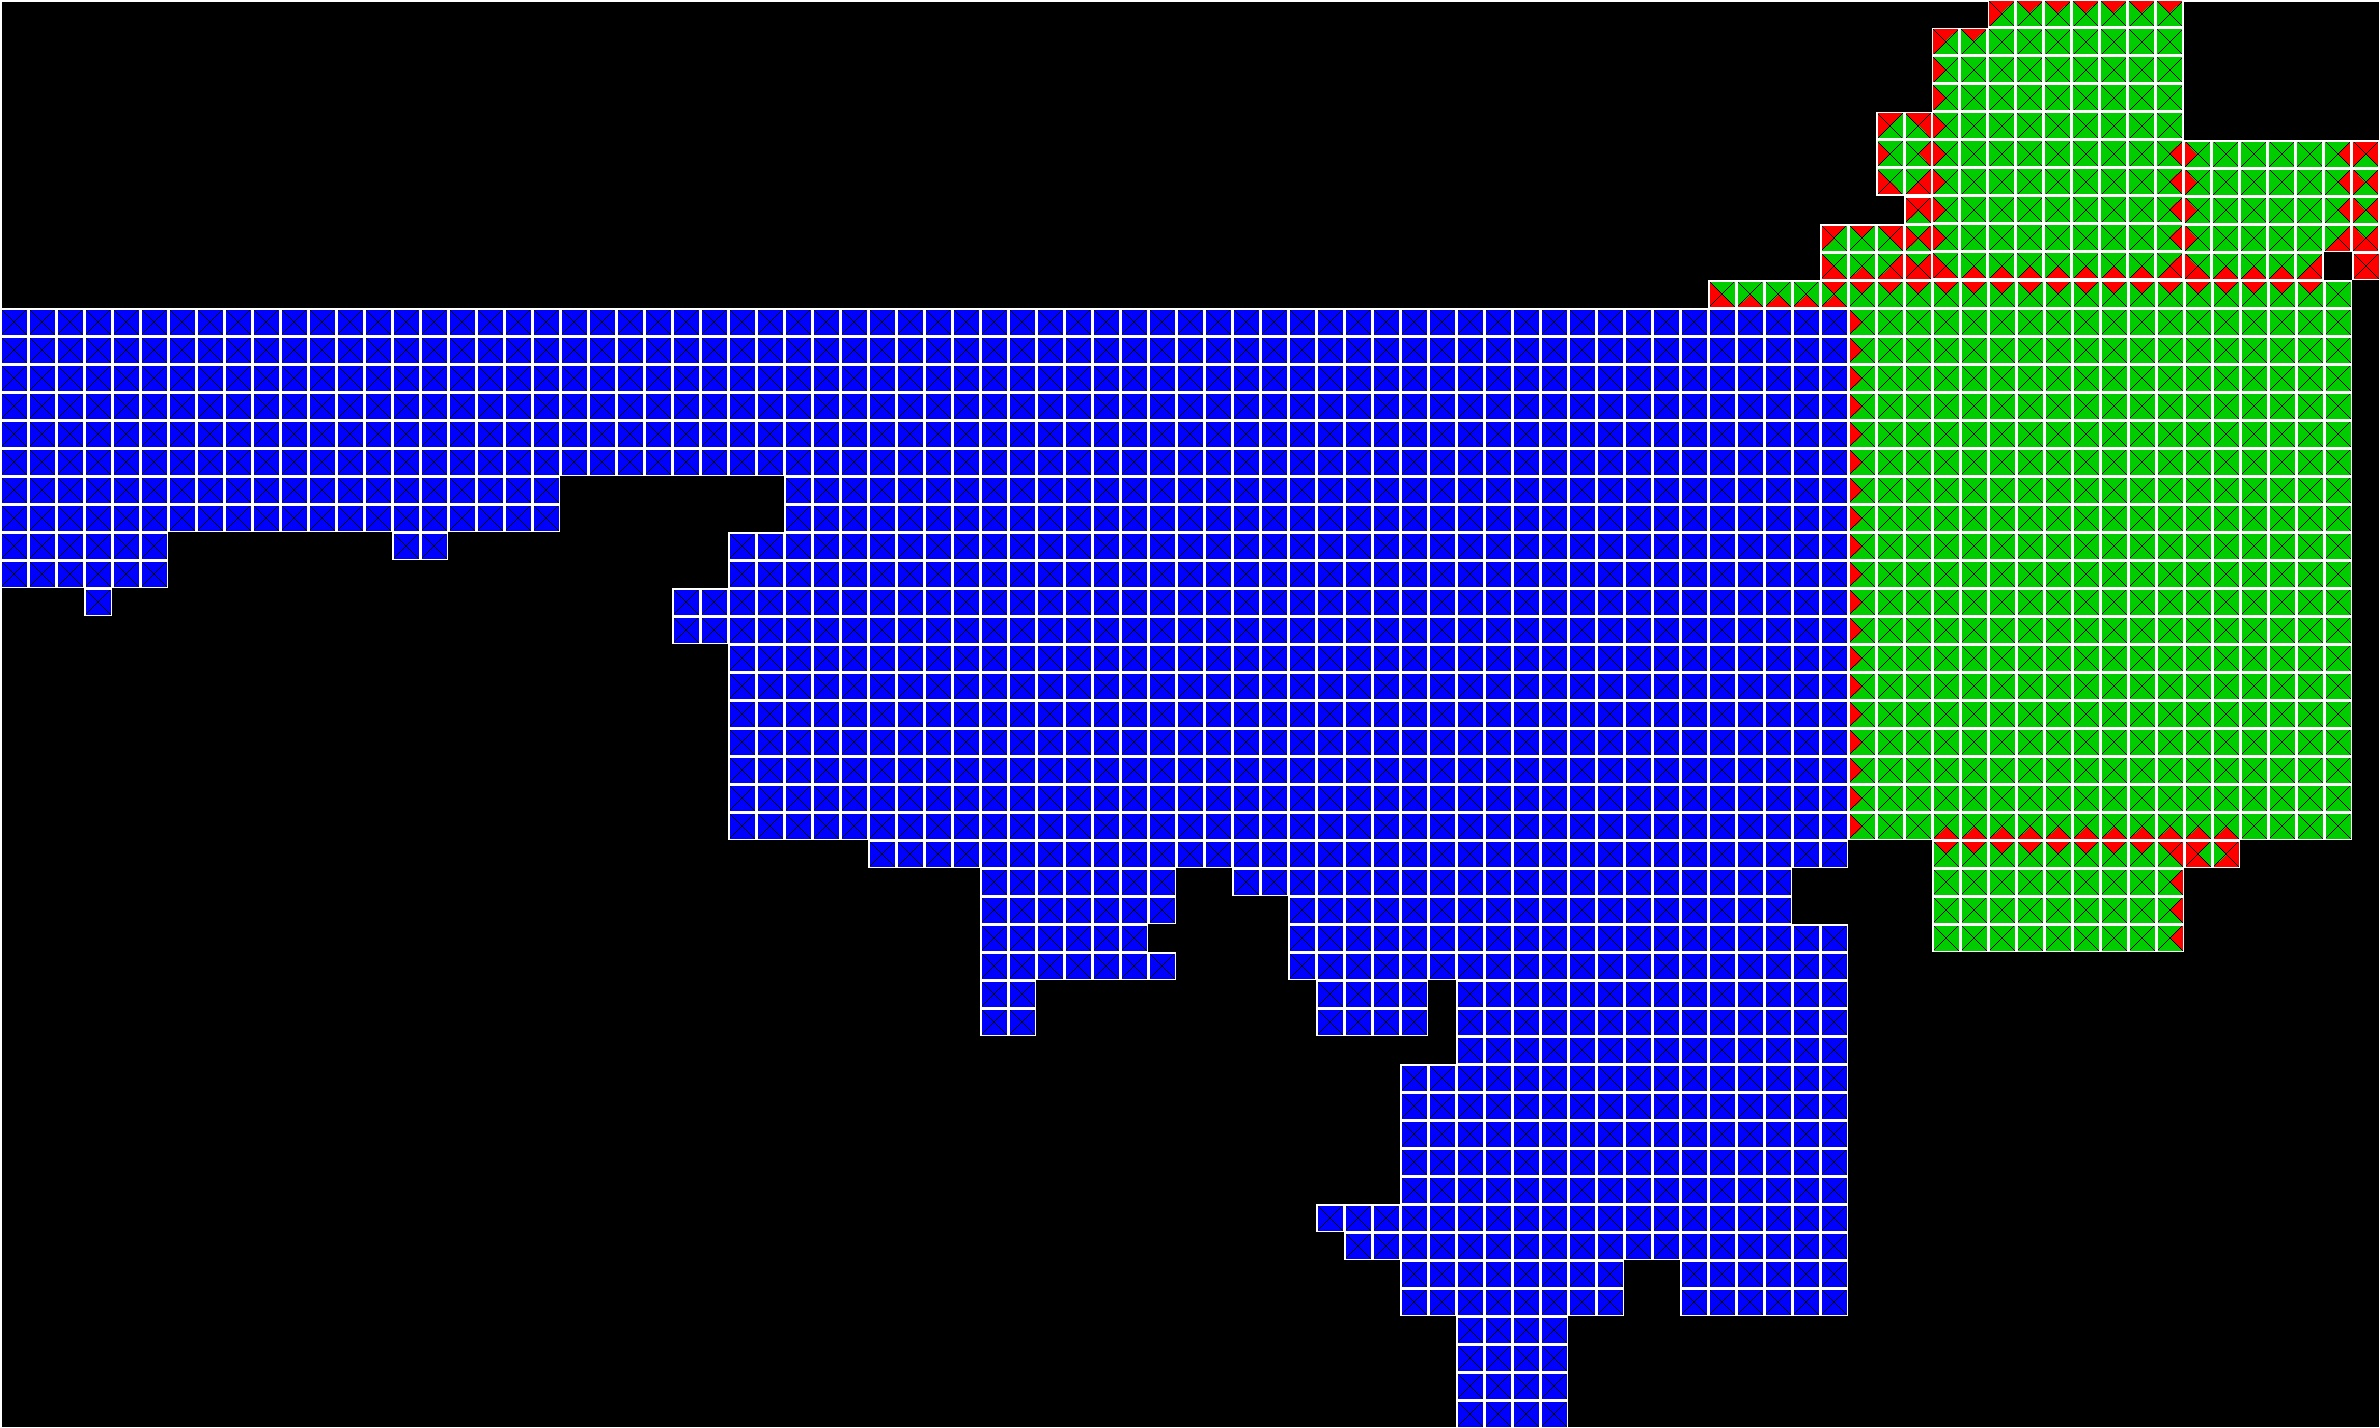
\includegraphics[width=2.1in]{./images/3300_1_mcgill_20_ENAS.jpg}}
\\~\\
	(c) Solver Output & (d) ENAS Visualization  
  \end{tabular}

\caption{Example Solver Output Visualization for ENAS}
\label{fig:neigborAccuracyVisualization}
\end{figure}

All pieces that came from the rainforest house image are shown as blue despite being assembled correctly; this is because they are not from the puzzle of interest.  All neighbors from the puzzle of interest (i.e., the glass and stone building) that are placed next to their original neighbor are represented by green triangles while all incorrect neighbors, such as those bordering the rainforest house image, are represented by red triangles.

\subsection{Visualizing Best Buddies}\label{sec:visualizingBestBuddies}

The visualization for best buddies is similar to that of neighbor accuracy.  Hence, each puzzle piece in the best buddy visualization is divided into four isosceles triangles with each triangle representing the piece's best buddy relationship with its neighbor.  Table~\ref{tab:bestBuddyColors} defines the color scheme used to denote the three best buddy relationships outlined in Section~\ref{sec:bestBuddyMetrics}.  


\begin{table}[t]
\begin{center}
  \begin{tabular}{ | >{\centering\arraybackslash}m{1.0in} | >{\centering\arraybackslash}m{1.0in} | >{\centering\arraybackslash}m{1.0in} | >{\centering\arraybackslash}m{1.0in} | }
  
   \hline
    No Best Buddy & Non-Adjacent Best Buddy & Adjacent Best Buddy & No Piece Present  \\ \hline
	{\cellcolor{white}~} & {\cellcolor{red}~} & {\cellcolor{green}~} & {\cellcolor{black}~}  \\
	{\cellcolor{white}~} & {\cellcolor{red}~} & {\cellcolor{green}~} & {\cellcolor{black}~}  \\
 \hline

  \end{tabular}
\end{center}
\caption{Color Scheme for Puzzles Piece Sides in Best Buddy Visualizations}\label{tab:bestBuddyColors}
\end{table}


\begin{figure}[t]
  \centering
  \begin{tabular}{ >{\centering\arraybackslash}m{2.2in} >{\centering\arraybackslash}m{2.2in} }
     \fbox{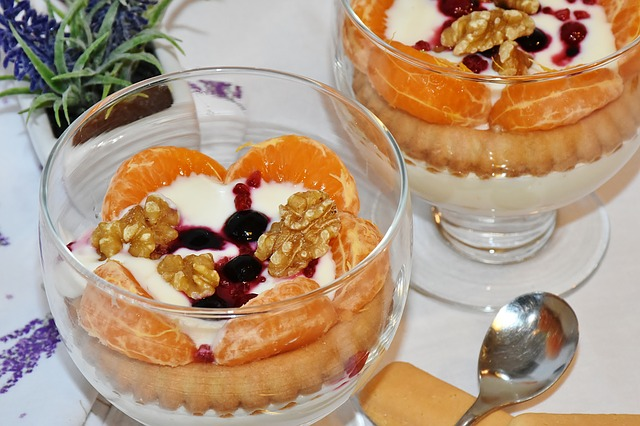
\includegraphics[width=50mm]{./images/dessert_pixabay.jpg}}  & \fbox{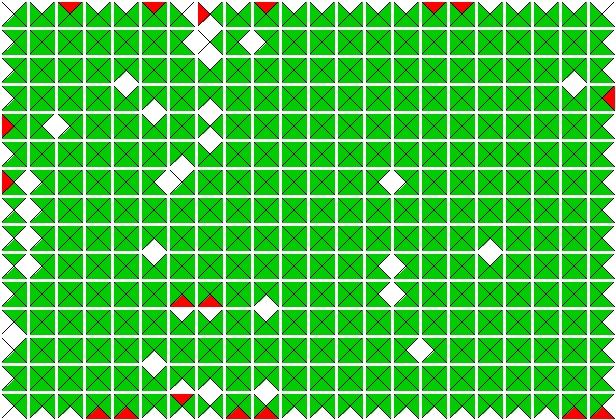
\includegraphics[width=50mm]{./images/dessert_best_buddy_visualization.jpg}}
     \\~\\
     (a) Original Image~\cite{pixabay} & (b) Best Buddy Visualization
  \end{tabular}
\caption{Visualization of Best Buddies in an Image}
\label{fig:bestBuddyVisualization}
\end{figure}

Figure~\ref{fig:bestBuddyVisualization} shows an example image and its best buddy visualization.  Note that the image has 4 interior and 14 exterior non-adjacent best buddies.  This is despite having 16-times more interior interior sides.  What is more, one can see that the best buddy density is high and generally uniform.